\section{Introduction}
The humanity instinctively feels a symbiotic relationship with the stars. One of the primary scientific projects of the humanity is to figure out what the stars are and how do they do what they do. The first obvious step in this project, beyond measuring their global parameters like diameter, mass, orbital and astromteric elements, is to obtain images of the stars with all details of the stellar surfaces as we do routinely in case of the Sun. In other words, the objective is to achieve capability of high fidelity image reconstruction of distant stars. Two interferometry based techniques, namely, Michelson Interferometry (MI) or Intensity Interferometry (II) have emerged during the last century to address this objective. A discussion of the development of these two approaches and comparison of their respective merits and challenges can be found in \citep{Rai2025}. The work reported here presents the results of a first effort at applying a conditional Generative Adversarial (neural) Network (cGAN) to image reconstruction of a fast rotator using its simulated II observations.  

The foundational basis of II stems from the pioneering experiments and theoretical investigations, widely referred to as the \textquotedblleft HBT effect \textquotedblright, carried out initially by Hanbury Brown and Twiss (HBT) \cite{HBT56Lab,brown1957interferometry, brown1958interferometry} and, later, by Glauber \citep{glauber1963quantum}. HBT reported \cite{HBT56Lab} in 1956, the correlation between photons measured by a pair of photon detectors in two coherent beams of light. Rai et al. \cite{Rai2025} present a modern-day variant of this experiment, carried out with pseudo-thermal light. The HBT Effect and the related theoretical investigations laid the foundation for the modern field of Quantum Optics.

Hanbury Brown and his collaborators led the creation and installation of the iconic II facility at Narrabri, Australia and reported the measurement of angular diameters of 32 stars and a few multiple star-systems \citep{hanbury1974angular}. Soon after this work, however, II observations of stars was stalled for over four decades due to the limits of the then available photon detectors and data processing equipment. With gradual mitigation of such issues, proposals to utilize Imaging Atmospheric Cherenkov Telescope (IACT) facilities for conducting II observations of stars have emerged\citep{LeBohec2006, nunez2010stellar, nunez2012high, 2013APh....43..331D} as a secondary science application of these facilities during moonlit nights. SII observations at VERITAS, MAGIC, and HESS are now being reported \citep[e.g.,][]{2024ApJ...966...28A,2024MNRAS.529.4387A,2025MNRAS.537.2334V}. This approach has the potential to enhance the scientific output of existing IACT facilities, and especially of the upcoming Cherenkov Telescope Array Observatory (CTAO). Simulations carried out by Rai et al. \citep[e.g.,]{10.1093/mnras/stab2391, 10.1093/mnras/stac2433} have shown that recent advancements in photon detectors could be effective in achieving high-precision measurements of parameters for stellar objects. 

The thrust of these efforts has been to measure the average global parameters of stars and star systems. The high fidelity imagery, however, would transcend the measurement of global and average stellar parameters, such as angular diameters, binary separations, and orbital characteristics, which offer only an integrated view of the star or star system as a whole. Such imaging capabilities promise direct insights into the dynamic surface phenomena, including limb darkening, convection cells, granulation, star spots, oblateness and gravity darkening in rapid rotators and atmospheric structures, akin to the detailed observations routinely conducted on our own Sun.

As it stands today, studies grappling various issues of image reconstruction are being reported \citep{Haubois2009, Norris2021AZCyg, Liu2024SuperresolutionII, Liu2025}. MI-based image reconstruction has made substantial progress in this area with efforts at generating constructed images of stars like Betelgeuse \citep{Haubois2009} and AZ Cyg \citep{Norris2021AZCyg}. On the other hand, II-based methods are in a nascent stage. The recent publications of Liu et al. \cite{Liu2024SuperresolutionII, Liu2025} have demonstrated, through outdoor experiments, imaging millimeter-scale targets at 1.36 km with a resolution ~14 times better than a single telescope’s diffraction limit. A \textquotedblleft flexible computational algorithm \textquotedblright reconstructs images from intensity correlations, overcoming atmospheric turbulence and optical imperfections. 

We report here, the results of our attempt, the first of its kind, to reconstruct the II-simulated gravity-darkened images of fast rotating stars using a cGAN neural network architecture. Image reconstruction in gravity darkened fast rotating stars has long been examined using various methods in MI \citep{vanBelle2001, DomicianodeSouza2003, DomicianodeSouza2005, Monnier2007, Pedretti2009, Zhao2009, Martinez2021}. Recently photosphere oblateness of $\gamma$-Cassiopeia \citep{2025arXiv250615027A} has been measured at the VERITAS observatory using II. These results, and especially, that by Archer et al. \cite{2025arXiv250615027A}  put our work in context. Thus our simulation is a natural next step of the work of Archer et al and others. We emulate the cGAN model of Isola et al. \cite{isola2017image} to reconstruct images of fast-rotating stars using their simulated Intensity Interferograms and simulated sky-intensity distributions as input data for training, testing, and validation. We consider four Imaging Cherenkov Telescope Arrays (IACTs) and simulate observation of a fast-rotating star. The image predicted by the trained GAN shows promising results in reconstructing the star’s shape and size. The reconstructed brightness distributions are then assessed using moments.

This paper is organized as follows. The next section discusses briefly the past efforts at image reconstruction on II, followed by the section on a discussion of Intensity Interferometry, focusing on its signal and noise characteristics for fast-rotating stars along the Earth’s rotation. The following section introduces the GAN formulation and its structure. The fifth section details the parameter selection for training the GAN for image reconstruction. The sixth section presents the results of the trained GAN both visually and via image moments. Finally, the paper concludes with a discussion of the overall results.
\begin{figure}
	\centering
	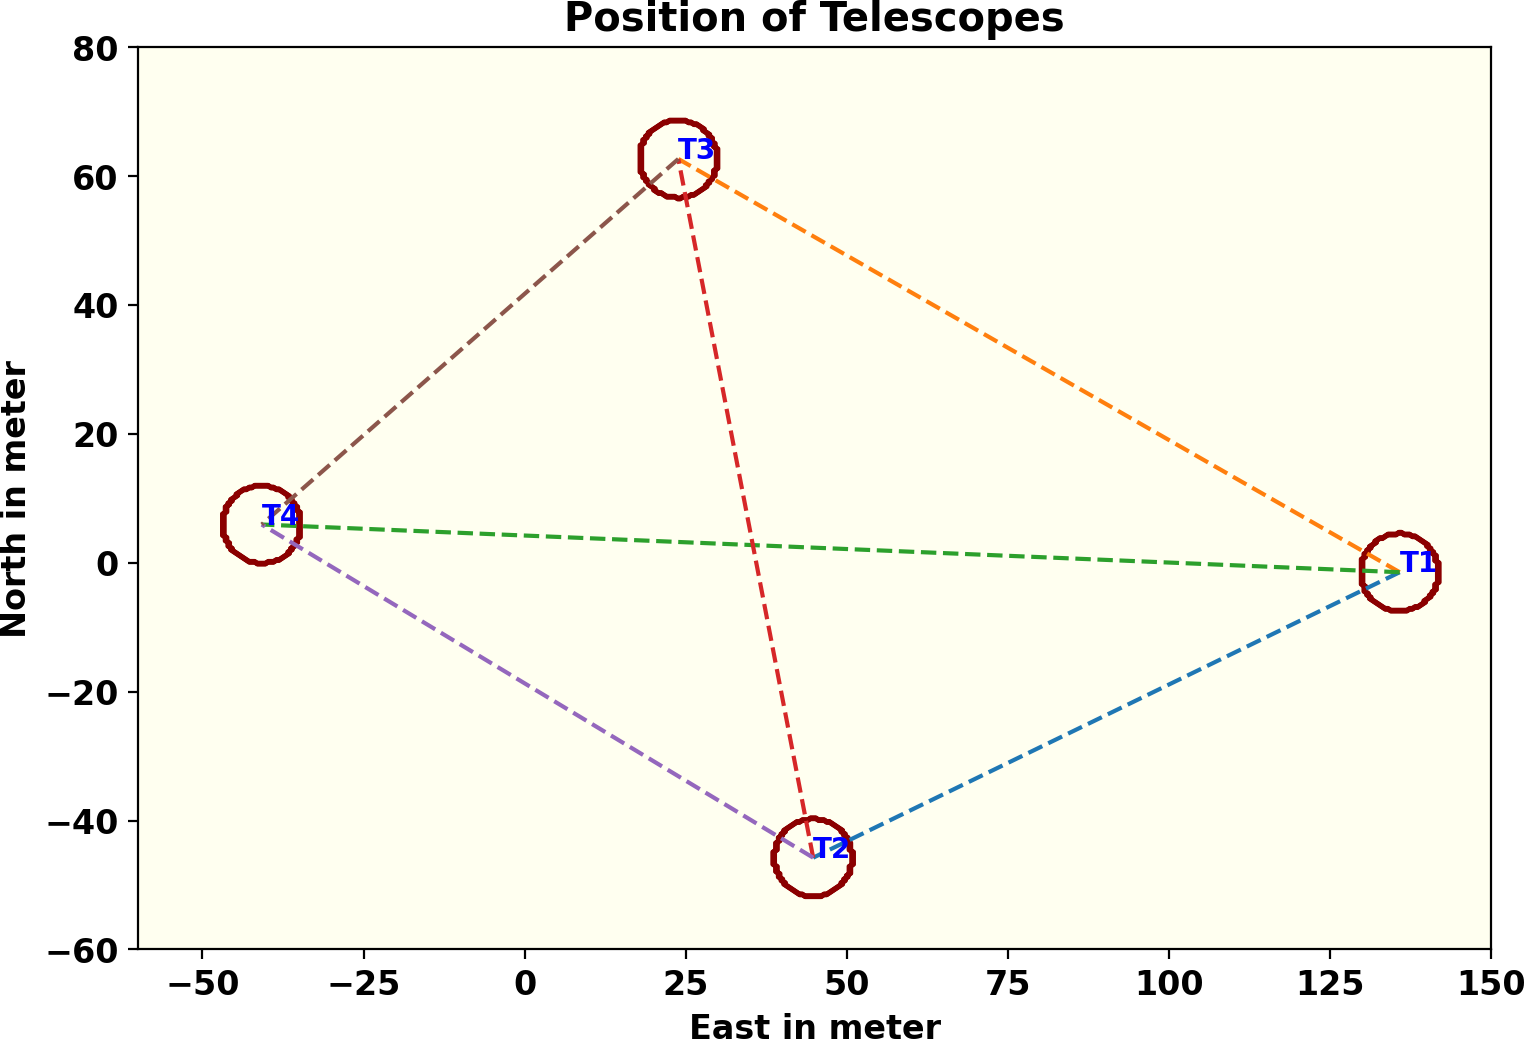
\includegraphics[width=\linewidth]{fig/telescope.png}
	\caption{The telescope configuration with similar properties each, where diameter is 12 meter and baselines are spreaded over more than 100 meter. This setup is used to simulate the signal for II observation.}
	\label{fig:teles}
\end{figure}